\begin{frame}{Ciencia de la computación}


\begin{block}{Ciencia}
\begin{itemize}
    \item La ciencia es un cuerpo de conocimiento organizado o sistemático. La ciencia abarca muchos dominios diferentes, sin embargo, esos dominios están relacionados. [1].
\end{itemize}
\end{block} 
        
\begin{block}{Ciencia de la computación}
\begin{itemize}
     \item Con respecto a la informática (CS), algunos dijeron que no debería llamarse ciencia.
    \item CS es transversal a dominios muy diferentes y es un gran tema de investigación científica.
\end{itemize}
\end{block}   
        

\end{frame}

\begin{frame}{Ciencia de la computación}
\begin{figure}[H]
    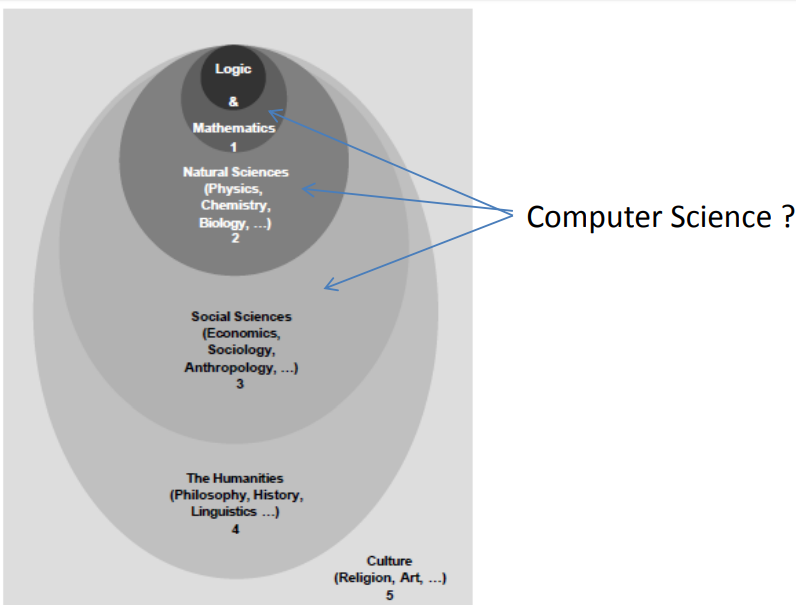
\includegraphics[scale=0.4]{images/figura1.PNG}
    \caption{Ciencia de la computación [1]}
    \label{fig:boat1}
\end{figure} 
\end{frame}

\begin{frame}{La Investigación}
\begin{block}{La investigación}
La investigación es un estudio cuidadoso, sistemático, paciente y una investigación en algún campo del conocimiento, realizado para establecer hechos. [1]
\end{block} 
\end{frame}


\begin{frame}{La Metodología}
\begin{block}{La metodología}
La metodología es la estrategia general que describe la forma en que se debe emprender el proyecto y, entre otras cosas, identifica los métodos que se utilizarán en él. [1]
\end{block} 
\begin{exampleblock}{}
\begin{itemize}
    \item Los investigadores de ciencias de la computación utilizan varias metodologías para abordar preguntas dentro de la disciplina. 
    \item Las tareas realizadas por un solo investigador se encuentran dentro de diferentes metodologías. Incluso las actividades requeridas para abordar una única pregunta de investigación pueden incluir varias de estas metodologías.
\end{itemize}
\end{exampleblock}
\end{frame}

\begin{frame}{Metodologías de búsqueda}
\begin{block}{Metodologías de la investigación. [2]}
\begin{itemize}
\item \textbf{En un contexto académico}: La investigación se utiliza para referirse a la actividad de una investigación o investigación diligente y sistemática en un área, con el objetivo de descubrir o revisar hechos, teorías, aplicaciones. 
\item [--] \textbf{El objetivo} es descubrir y difundir nuevos conocimientos. (existen varios métodos que se pueden usar en CS en la siguiente diapositiva que mostraremos estas metodologías).
\end{itemize}
\end{block} 
\end{frame}

\begin{frame}{Métodos que se pueden usar en Ciencia de la Computación}
\begin{figure}[H]
    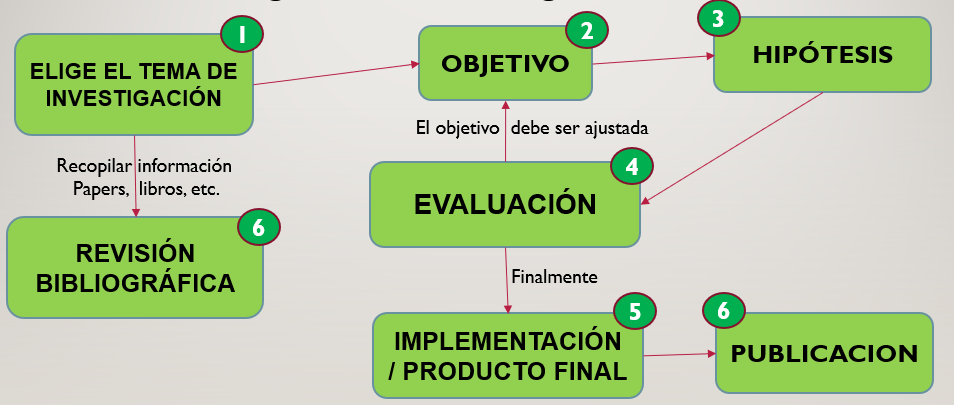
\includegraphics[scale=0.48]{images/figura3.PNG}
    \label{fig:boat1}
\end{figure}     
\end{frame}

\begin{frame}{Diagrama2 : Metodologías científicas en Cs}
 \begin{figure}[H]
    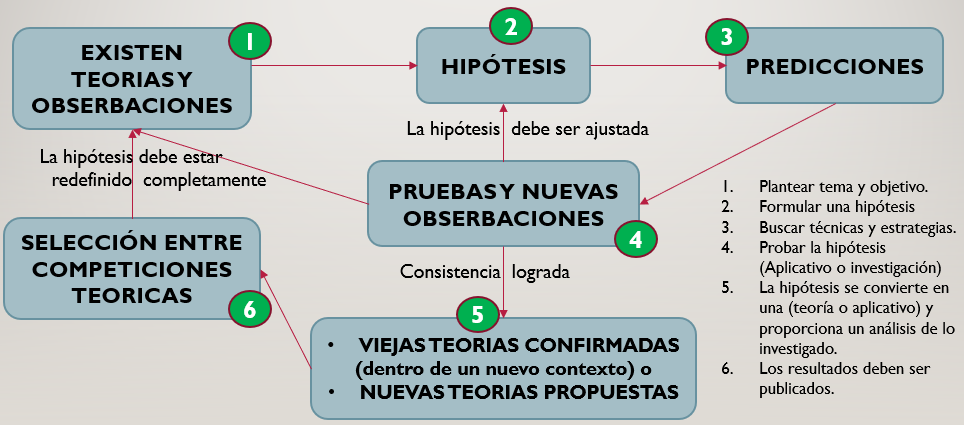
\includegraphics[scale=0.48]{images/figura5.PNG}
    \label{fig:boat1}
\end{figure}    
\end{frame}